% !TEX root = ../main.tex

\section{Context}
\begin{frame}{\insertsec}
	\begin{itemize}
    \item Nowadays Machine Learning is widely used
    \item Medical images can be obtained using MRI, PET or CT scans but are underused
    \item Different methods have appeared to analyze these data for image classification,
    object detection, segmentation...
    \item Deep learning models aim to be able to unlock the full potential of medical imaging
    \item Hand-crafted radiomic features can be extracted from medical images
    \item The work will be centered around predicting patients' survival
  \end{itemize}
\end{frame}

\subsection{Survival Analysis}
\begin{frame}{\insertsubsec}
  Survival analysis models usually have:
  \begin{itemize}
    \item Baseline data \( x \)
    \item Event \( E \in \{0, 1\} \)
    \item Time \( T \)
    \item Censoring
  \end{itemize}
  
  Survival function:
  \[
    S(t) = \Pr(T \ge t)
  \]

  Hazard function:
  \[
    \lambda(t) = \lim_{\Delta t \rightarrow 0}
    \frac{\Pr(t \le T < t + \Delta t | T \ge t)}{\Delta t}
  \]
\end{frame}

\begin{frame}

  Casting the survival problem as a ranking is a way of dealing with censored data.
  Conditions:
  \begin{itemize}
    \item Both of them are uncensored (\( \bm{E}_i = \bm{E}_j = 1\))
    \item The uncensored time of one is smaller than the censored survival time of the other
    (\( \bm{T}_i < \bm{T}_j | \bm{E}_i = 1; \bm{E}_j = 0 \))
  \end{itemize}

  \begin{columns}
    \begin{column}{.5\textwidth}
      \begin{figure}
        \centering
        \scalebox{.8}{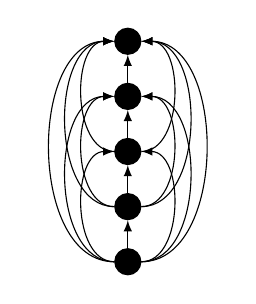
\begin{tikzpicture}[scale=.7]
  \tikzstyle{bDot}=[circle, fill=black, draw]
  \foreach \y in {1,...,5} {
    \node[bDot] (D-\y) at (0, \y) {};
  }

  \foreach \y in {1,...,4} {
    \pgfmathsetmacro{\z}{int(\y + 1)}
    \draw[-latex] (D-\y) -- ({D-\z}.south);
  }

  \foreach \y in {1,...,3} {
    \pgfmathsetmacro{\z}{int(\y + 2)}
    \foreach \j in {\z,...,5} {
      \ifthenelse{\y=2 \OR \y=3}{
        \draw[-latex] (D-\y) to[bend left=90] (D-\j);
      }{
        \draw[-latex] (D-\y) to[bend right=90] (D-\j);
      }
    }
  }
\end{tikzpicture}
}
        \caption{Uncensored data}
      \end{figure}
    \end{column}
    \begin{column}{.5\textwidth}
      \begin{figure}
        \centering
        \scalebox{.8}{\begin{tikzpicture}
  \foreach \y in {1,...,5} {
    \ifthenelse{\y=2 \OR \y=4}{
      \node [circle, fill=white, draw=black] (D-\y) at (0, \y) {};
    }{
      \node [circle, fill=black, draw=black] (D-\y) at (0, \y) {};
    }

    \foreach \y in {3,4,5} {
      \draw [-latex] (D-1) to[bend right=90] (D-\y);
    }

    \foreach \y/\z in {1/2, 3/4} {
      \draw [-latex] (D-\y) -- (D-\z);
    }
    \draw [-latex] (D-3) to[bend left=90] (D-5);
  }
\end{tikzpicture}
}
        \caption{Censored data}
      \end{figure}
    \end{column}
  \end{columns}
\end{frame}

\begin{frame}
  \begin{block}{Good prediction}
    \[
      T_i > T_j \land \hat{T}_i > \hat{T}_j
    \]
  \end{block}

  \begin{block}{Bad prediction}
    \[
      T_i > T_j \land \hat{T}_i < \hat{T}_j
    \]
  \end{block}

  \begin{block}{Concordance Index}
    \[
      CI = \frac{\text{Good predictions}}{\text{Total predictions}} \in [0, 1]
    \]
  \end{block}
\end{frame}

\subsection{Dataset}
\begin{frame}{\insertsubsec}
  \begin{itemize}
    \item Dataset with 671 patients diagnosed of Oropharyngeal Squamous Cell Carcinoma
    \item CT scan of \( 512 \times 512 \) with 100-200 slices
    \item Tumour annotated in provided mask
    \item Clinical information compressed of:
    \begin{itemize}
      \item Subject characteristics
      \item Tumour characteristics
      \item Treatment data
      \item Outcome data
    \end{itemize}
  \end{itemize}
\end{frame}

\begin{frame}
  \begin{figure}
    \centering
    \begin{subfigure}[t]{.32\textwidth}
      \centering
      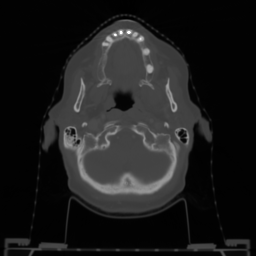
\includegraphics[width=\textwidth]{images_main/IMG0138_example.png}
      \caption{Original image}
    \end{subfigure}
    \hfill
    \begin{subfigure}[t]{.32\textwidth}
      \centering
      
\includegraphics[width=\textwidth]{images_main/IMG0138_MASS_example.png}
      \caption{Image mask}
    \end{subfigure}
    \hfill
    \begin{subfigure}[t]{.32\textwidth}
      \centering
      
\includegraphics[width=\textwidth]{images_main/IMG0138_merge_example.png}
      \caption{Mask applied to original}
    \end{subfigure}
  
    \caption[Images from the dataset]{
      Example of images from the dataset
    }
  \end{figure}
\end{frame}

\subsection{Neural Networks}
\begin{frame}{\insertsubsec}
  \begin{figure}
    \centering
    
\tikzset{
  pics/layer/.style n args = {3}{
    code = {
      \foreach \y in {1,...,#1} {
        \node[draw, circle] (L-#2-\y) at (0,{1.5*(\y - #1/2)}) {${#3}_{#2 \y}$};
      }
    }
  }
}

\begin{tikzpicture}
\def\layers{2/I, 5/H, 5/H, 3/O}

\foreach \x/\name [count=\xi] in \layers  {
  \draw (3*\xi, 0) pic {layer={\x}{\xi}{\name}};
}

\foreach \x/\ignore [count=\xi, remember=\xi as \lastxi, remember=\x as \lastx] in \layers {
  \ifthenelse{\xi > 1}{
    \foreach \ylast in {1,...,\lastx} \foreach \y in {1,...,\x}{
      \draw [-latex] (L-\lastxi-\ylast) -- (L-\xi-\y);
    }
  }{};
}

\end{tikzpicture}


    \caption[Neural network graph]{
      Neural Network graph drawing. 
    }
  \end{figure}
\end{frame}

\begin{frame}
  \begin{block}{Hidden Layers}
    \begin{equation*}
      \begin{aligned}
        z_i^{[l]} &= \sum_{j = 1}^{n^{[l]}} w_{ij}^{[l]} + w_{i0}^{[l]} \cdot a_j^{[l - 1]} \\
        a_i^{[l]} &= g^{[l]}(z_i^{[l]})
      \end{aligned}
      \quad
      \xrightarrow{\text{becomes}}
      \quad
      \begin{aligned}
        \bm{z}^{[l]} &= \bm{W}^{[l]} \cdot \bm{a}^{[l - 1]} + \bm{b}^{[l]} \\
        \bm{a}^{[l]} &= g^{[l]}(\bm{z}^{[l]})
      \end{aligned}
    \end{equation*}
  
  \end{block}
  \begin{figure}
    \centering
    
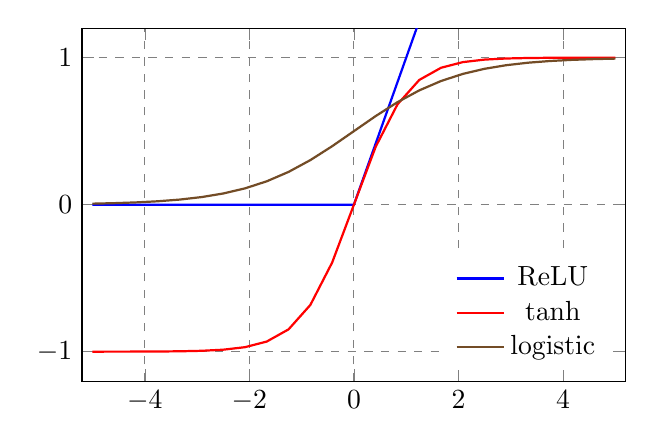
\begin{tikzpicture}
\begin{axis}[
    xmin = -5.2, xmax = 5.2,
    ymin = -1.2, ymax = 1.2,
    legend style = {draw = none},
    legend pos = south east,
    grid=major,
    grid style = {dashed, gray},
    width = 0.7\textwidth,
    height = 0.5\textwidth,
    every axis plot/.append style={thick},
    no markers,
    cycle list name = color
  ]
  \addplot{max(0, x)};
  \addplot{tanh(x)};
  \addplot{1/(1 + exp(-x))};
  \legend{ReLU, tanh, logistic}
\end{axis}
\end{tikzpicture}
  
    \caption[Activation functions]{
      Activation functions
    }
  \end{figure}
\end{frame}

\begin{frame}
  \begin{block}{Output layers}
    \[
      g_k^{[L]}(\bm{a}^{[L - 1]}) = \frac{e^{a_k^{[L - 1]}}}{\sum_{i = 1}^K e^{a_i^{[L - 1]}}}
    \]
  \end{block}
  
  \begin{block}{Cost function}
    \begin{align*}
      \hat{\bm{y}} &:= g^{[L]}(\bm{a^{[L - 1]}}) \\
      C(\bm{y}, \hat{\bm{y}}) &:= \frac{1}{N} \sum_{i = 1}^N (y_i - \hat{y}_i)^2
    \end{align*}
  \end{block}
\end{frame}

\subsection{Convolutional Neural Networks}

\begin{frame}{\insertsubsec}
  \centering
  \begin{figure}
    \hspace{-7cm}
    \adjustbox{max width=1.35\pagewidth}{\input{drawings/convolution_operation.tikz.tex}}

    \caption{Convolution operation}
  \end{figure}

  \begin{block}{Output size}
    \begin{align*}
      n_{\text{next}} = \left\lfloor\frac{n_{\text{prev}} + p - f}{s}\right\rfloor + 1
    \end{align*}
  \end{block} 
\end{frame}

\begin{frame}
  \begin{figure}
    \centering
    \scalebox{.7}{\input{drawings/convolutional_layer.tikz.tex}}
    \caption{Convolutional layer}
  \end{figure}

  \begin{align*}
    \bm{z}^{[l]} &= \bm{W}^{[l]} \cdot \bm{a}^{[l - 1]} + \bm{b}^{[l - 1]} \\
    &\downarrow \text{becomes} \\
    \bm{\mathsf{Z}}^{[l]} &= \bm{\mathsf{A}}^{[l - 1]} * \bm{\mathsf{W}}^{[l]} + 
    \bm{\mathsf{B}}^{[l - 1]}
  \end{align*}
\end{frame}
